
\chapter{标签同步解码的扩展应用}

本章节我们将进一步探讨标签同步解码算法的一些扩展应用。这包括置信度框架,多识别任务统一框架,以及端到端语音识别。

由于不同ASR应用之间不同的搜索空间大小和效率要求,当前业界最优的置信度及其相应的解码算法在不同应用上具有不同架构,这些不同应用包括:关键词检测,基于上下文的语音识别和大词汇连续语音识别。针对基于词图后验概率的置信度,计算量主要集中在词图部分的边缘概率计算过程。如第~\ref{chap:intro2-dec-todo}章节中对于解码搜索的研究机遇的讨论,本章节中,我们将结合前面章节对解码的大幅加速和搜索空间的优化等工作,提出一系列针对不同应用的通用置信度,并尝试将不同应用中的语音识别推理搜索过程统一到同一框架中。
本章节所提出的置信度在Switchboard数据集上得到了显著改善,同时这类统一框架的通用置信度在不同应用中取得了一致的非常有竞争力的性能,使得各种语音识别应用可以工作在同一框架中。

另一方面,该章节研究将标签同步算法应用于序列到序列的端到端模型的方案。在实验部分,该章节系统一方面取得大幅度语音识别解码速度改善,另一方面在端到端建模上取得了更快和更好的模型收敛和模型准确度。

\section{基于标签同步解码的置信度框架}
\label{chap:unify-confidence}


连接时序分类模型 (CTC) 是一种目前比较主流的LVCSR模型。但是由于 $\tt blank$ 的引入,使得基于 CTC的词语级别的置信度 (CM) 并不能够被直接得到,特别是最主流的针对传统基于音素似然度归一化或者基于词图后验概率的混淆网络等方法。
在前文中我们提出了标签同步解码(LSD)的推理搜索框架,它的主要作用是针对CTC或HMM模型进行高效的解码搜索。该算法提出了一些方式来自动地将 $\tt blank$ 帧进行忽略,由此不仅得到了搜索上的加速,还得到了一种非常紧致高效的 CTC 音素词图。在这项工作中,两种置信度生成算法在标签同步解码算法的基础上被提出。
更细致的研究显示这种基于CTC的音素词图是得到更好性能的关键所在。
在英文Switchboard 上的大词汇连续语音识别任务显示这里提出的LSD CTC 词图置信度算法可以显著改善原先传统的基于逐帧解码算法的CTC置信度或者 HMM模型的置信度。

\subsection{语音识别中的置信度}
\label{sec:intro}

% TODO: ref http://hci.stanford.edu/research/speech/
在最近十年时间,自动语音识别 (ASR) 取得了非常显著的成功。但是当语音识别系统由实验室产品转向真正的应用时,即使是最好的语音识别系统,仍然会不可避免地产生一些识别中的错误 \cite{ruan2016speech},也就是说ASR系统的输出总会包含或多或少的一些各种各样的错误。
因此,在真实的应用场景中,人们一般需要ASR系统能够自动评估自身的可靠性和发生错误的概率,而这些都由系统自身得出。

在语音识别中,置信度(CM)就是提出来进行这种类型的可靠度评估的\cite{jiang2005confidence}。这类模型可以被分为如下几种类别:

\begin{itemize}
    \item {\em 基于用于建模的特征的置信度}.
    基于ASR识别过程的特征被称为用于建模的特征,而它的概率分布在识别正确和识别错误时会产生显著的不同。
    CM可以由它们之中的一个或两个来组成,比如对归一化后的声学分数 \cite{hu2013new}, 时长 \cite{ma2011fusing}, 局部交叉熵 \cite{falavigna2002acoustic}。
    但是,这些用于建模的特征并不完美地表示解码的过程 \cite{jiang2005confidence}. 所以一些分类器模型也可以考虑被加入到这些用于建模的特征上,比如 CRF \cite{seigel2013confidence}, 深度学习 \cite{yu2011calibration}, 等等。但是这些模型仍然不够完美。首先各个用于建模的特征之间并不完全独立,其次它需要额外的训练阶段,并假设训练数据与测试数据匹配。
    %feature and model method weakness:
    %need further training stage; hard to formulate; depend on scenario of training data, assuming scenario of test and training data is the same

    \item {\em 基于后验概率的置信度}.
    另一种方法将ASR过程建模为 {\em 最大后验概率} (MAP) 的决策过程。给定整个句子后的ASR输出的后验概率可以用来表示CM。许多方法研究了如何对归一化项进行建模,比如 filler 模型 \cite{young1994detecting}, 词图\cite{wessel2001confidence} 和混淆网络 \cite{evermann2000large}。然而,ASR解码器通常设计用于寻找最优的首选路径,这使得它所得到的词图并不完美,同时会导致CM的建模并未较好地归一化 \cite{yu2006maximum}.
    %filler/lattice/cn

\end{itemize}

%review CTC & LSD & its potential in CM
CTC\cite{graves2006connectionist} 被提出来并作为目前主流的新模型\cite{fernandez2008phoneme}\cite{sainath2015acoustic}\cite{amodei2015deep}\cite{sak2015fast}.
同时,上下文无关的单音素CTC也显示出非常有竞争力的性能,在相比传统上下文相关的聚类混合深度学习HMM模型\cite{sak2015fast}\cite{miao2015eesen}\cite{miao2016ctc}\cite{mcgraw2016personalized}的情况下。
然而,由于引入了$\tt blank$, CM的计算亟待研究。如本文的实验部分所示,如果只是将 $\tt blank$ 标签当做一个特殊的音素并使用传统的CM方法,将会引入较大的性能下降。
在前文中我们提出了标签同步解码(LSD)的推理搜索框架。它的主要作用是针对CTC模型进行高效的解码搜索。该算法提出了一些方式来自动地将 $\tt blank$ 帧进行忽略,由此不仅得到了搜索上的加速,还得到了一种非常紧致高效的 CTC音素词图。在这项工作中,两种置信度生成算法在标签同步解码算法的基础上被提出。
更细致的研究显示这种基于CTC的音素词图是得到更好性能的关键所在。
在英文Switchboard 上的大词汇连续语音识别任务显示这里提出的LSD CTC 词图置信度算法可以显著改善原先传统的基于逐帧解码算法的CTC置信度或者 HMM模型的置信度。


\subsection{LSD CTC词图中的置信度}
\label{sec:pp-conf-measure}


\subsubsection{标签同步的音素声学置信度}
\label{sec:psd-ac-conf}

%as local confidence
在前文中,我们已讨论了标签同步解码算法,它的主要作用是针对CTC模型进行高效的解码搜索。该算法提出了一些方式来自动地将 $\tt blank$ 帧进行忽略,由此不仅得到了搜索上的加速,还得到了一种非常紧致高效的 CTC音素词图。
下面我们将集中讨论基于这些 CTC音素词图如何得到较好的置信度。

这里CTC音素后验概率可以依据词语进行区分,属于同一个词的后验概率可以用于一起对一个特定词在词图中出现的后验概率进行建模。
在LSD框架中,词级别的 CM $\mathcal{C}(w)$ 可以被定义为对数域的后验概率,针对其相应的最优路径。
% introduction of phonemic confidence


     \begin{equation}\label{eq:psd-ac-conf1}
        \mathcal{C}(w)  =
         \log\!\!\!\!\!\!\sum_{\bm\pi \in \mathcal{B}^{-1}(\mathbf{l}_w)}{\!\!\!\!\!\!P(\bm\pi|\mathbf{x})}
        \triangleq
   \!\!\!\!\!\!\mathop{\max}\limits
       _{\!\!\!\!\pi':\pi' \in L, \mathcal{B}(\pi'_{\mathbf{j}_w})       =       {\mathbf{l}}_w}
   \sum_{j:j\in \mathbf{j}_w}
   \log({y^{t_{j}}_{\pi'_{j}}})
     \end{equation}

$\mathbf{l}_{w}$ 表示词语  $w$对应的音素序列。
$j$ 是音素序列的索引 (i.e.  \cite{zhc00-chen-tasl2017}中定义的非$\tt blank$ CTC 标签序列).
由于LSD CTC中的词边间比较确定, $\mathbf{j}_w$ 可以被定义为 $w$ 词所最佳对应的音素序列索引。
我们提出的基于标签同步解码的声学分数可以作为单独的置信度,也可以与其他用于建模的特征结合,作为置信度模型的输入 \cite{yu2011calibration}。 
具体来说,$\mathcal{B}$函数的建模在CTC中并不完美,使得这里会出现同一个音素有多帧的音素后验概率输出。所以,我们需要在它上面进一步进行归一化。 其中一种方法是进行算数平均,被称为 {\em peak-mean}。但是,由于有多个概率输出尖峰,更好的一种方法是忽略不完美的部分并保留最大的结果,所以从中挑选最大的后验概率作为其置信度,被称为 {\em peak-max}。除此之外,不同词语具有不同的长度,因此我们需要针对长度作一次平均。为了使性能更好,我们这里对音素序列的长度也进行了归一化 称为{\em phone-mean}。

% introducing (no blk) confidence
另一类比较现实的问题是, {$\tt blank$} 的区段和音素区段有所重合。因此这里需要对非$\tt blank$的概率同样进行一些建模。音素置信度 (称为 {\em phone-conf }) 可以被定义为某帧上输出音素标签的概率。
%, in proposed CM (\ref{eq:psd-ac-conf1})
% \begin{equation}\label{eq:nblk-conf}
%    P( \tt phone^{t} |\mathbf{x}) = 1-y^{t}_{\tt{blank}}
%     \end{equation}
以上这些针对不同模块的设计总结如下 (\ref{eq:psd-ac-conf2}),

     \begin{equation}\label{eq:psd-ac-conf2}
        \mathcal{C}(w)
        \triangleq
        \!\!\!\!\!\!\mathop{\max}\limits
       _{\!\!\!\!\pi':\pi' \in L, \mathcal{B}(\pi'_{\mathbf{j}_w})       =       {\mathbf{l}}_w}
   \frac{1}{|\mathbf{j}_w|}\sum_{j:j\in \mathbf{j}_w}
   \max_{t:t\in\mathbf{t}_j}
   {\log(y^{t}_{\pi'_{j}}(1-y^{t}_{\tt{blank}})^\alpha)}
     \end{equation}
这里的 {\em peak-max} 作为一个例子出现在公式中。 $\mathbf{t}_j$ 是音素 $j$ 在最优路径下所相应的帧。 $\alpha$ 是置信度融合的权重概率。

%  \begin{equation}\label{eq:psd-ac-conf2}
%        CM(w)
%        =
%   PN(FN(\mathbf{t}_j,y\cdot(1-y_{\tt{blank}})),\mathbf{j}_w)
%     \end{equation}

\subsubsection{基于混淆网络和CTC标签同步解码词图的置信度}
\label{sec:psd-cn-conf}

类似于 \cite{evermann2000large}中的做法,这里生成混淆网络主要有两步: a) 从音素级别的标签同步CTC音素词图(图~\ref{fig:ctc-lat-exp})中产生词级词图; b) 将词级词图转换为混淆网络,利用其包含的时间边界信息。在 \cite{hakkani2006beyond}中提出的 pivot clustering 算法使得混淆网络生成复杂度为 $O(n)$ , $n$ 为词图的边数。在这项工作中,我们将最优路径视为pivot, 由于CTC词图非常紧致,因此  CN 产生的过程非常高效。在CN的构建过程中, 我们需要计算词后验概率,而其自然地成为了词级置信度。



\begin{figure}[tbhp!]
        \centering
        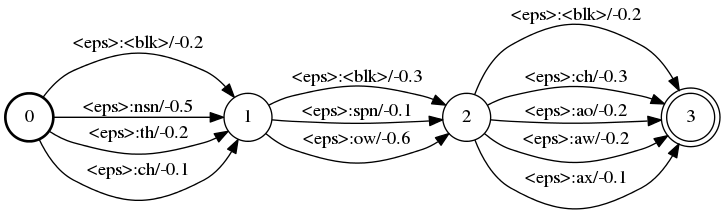
\includegraphics[width=0.95\linewidth]{figure/ctc_lat.png}
        \caption{{\it  LSD CTC Lattice的例子}}
        \label{fig:ctc-lat-exp}
      \end{figure}

图~\ref{fig:lat-exp} 中是一个真实的例子 (句子为 "OH YEAH") 表示了LSD CTC 产生的CN的高效性,以及与HMM-DNN产生的词图之间的比较。
由HMM和CTC得到的推理搜索结果在图~\ref{fig:lat-exp}(a)中进行显示,其得到的音素词图,词级词图,分别在HMM和CTC系统中展示于图~\ref{fig:lat-exp}(b$\sim$e)中。我们可以观察到,CTC基于LSD得到的音素词图和词级词图比相应的HMM词图更加紧致,这是源于$\mathcal{B}$函数的建模结果。另一方面,HMM的词图需要额外的启发式方法来进行多对一的映射,以便去除词图冗余性。这里的做法是进行词图裁剪 \cite{siniscalchi2013bottom}, 而它不如 $\mathcal{B}$ 函数的效果那么强。
另一方面,当CTC模型被使用于传统的 {\em 逐帧同步解码} (FSD) 框架时, 音素和词级词图可以由同样方法进行产生\cite{povey2012generating},类似于处理 HMM-DNN 词图的方式对 $\tt blank$ 标签进行等同于音素的处理。但是由于逐帧搜索和词图此案件所带来的搜索误差,以及词图边界的混淆性,所得到的CN将会具有更差的质量。我们将会在后续的实验章节中进行详细比较。

%FSD Lattice v.s. LSD Lattice
%
%snt example fig:
%ref word v.s. phn dnn align v.s. phn dnn decode v.s. phn CTC align v.s. phn CTC decode
%v.s. FSD lattice v.s. LSD lattice v.s. CN
%in a single figure

%analysis on latter indicators in experiment part

\begin{figure}[tbhp!]
        \centering
        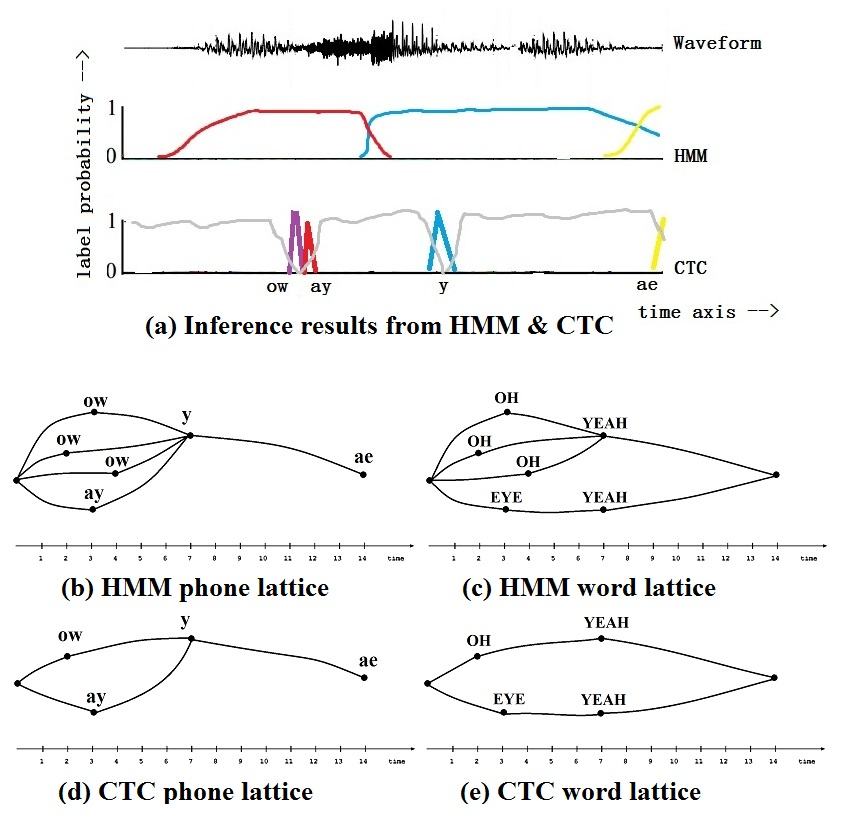
\includegraphics[width=0.95\linewidth]{figure/lat-exp.jpg}
        \caption{{\it FSD HMM 和 LSD CTC所产生的词图比较}}
        \label{fig:lat-exp}
      \end{figure}

\section{基于标签同步解码的多识别任务统一框架}
\label{chap:unify-framework}

要为所有的ASR应用设计一套统一的推理搜索框架,并取得最好的性能和速度,是一项非常有挑战的研究。这里面的关键点在于: i) 如何对最佳识别结果进行规范化,以得到对该最佳结果的置信度估计,也就是置信度中的归一化项的建模
    ii) 如何保证在低功耗设备中的计算量控制在一个较小范围内,比如关键词检测技术就经常被用于个人助理情况,需要对功耗进行优化。
    {\em Keyword-filler}方法~\cite{young1994detecting} 和 {\em utterance verification}~\cite{rose1995training} 方法都可以视为这方面的尝试。比如,在关键词检测中,一些研究提出使用上下文无关的(CI) 语言学单元,称为 $\tt filler$ 来对所有非关键词部分进行建模,而这种建模往往是不完美的。
    在基于上下文的语音识别中,这种框架更加受制于较弱的上下文建模能力,而这将影响 $\tt filler$ 的识别效果。
    %More elaborated $\tt filler$~\cite{el1997accurate}, e.g., CD $\tt filler$, is proposed to improve the recognition but brings about further computational burden without significant improvement.
    在LVCSR中,理论上更好的办法是基于识别结果的后验概率方法的置信度~\cite{wessel2001confidence}, 也就是前文讨论的第二种置信度。 在这种置信度里,ASR被建模为  {\em maximum a posterior} (MAP) 过程:给定句子,求取当前识别结果的后验概率,并将其作为置信度。而这里的观察概率(归一化项)使用针对搜索空间的所有可能候选概率求和来得到。由于ASR搜索空间很大,词图建模很耗时。在LVCSR中,这种框架往往取得最好的效果,但在其他任务中结论不尽相同。

    最近在鉴别性训练领域,有些研究采用一个特别设计的音素语言模型作为搜索空间来代替词图,该方法显示出了较好的性能~\cite{chen2006advances}\cite{povey2016purely}。受次启发,我们尝试将这样的音素语言模型应用到置信度的归一化项的建模当中,由此我们提出了辅助归一化搜索空间的概念。我们尝试使用这样的搜索空间来建模所有ASR应用领域的置信度。 % and CM can be obtained in an unified framework
    而针对这样做在低功耗设备上带来的挑战,我们采用基于CTC的标签同步解码\cite{Chen+2016} 来进行处理,由此带来了很大的效率改善。
    由此我们提出了一个统一并且高效的置信度框架,并且将其应用于目前主流的上述三种 ASR应用。

  \subsection{置信度与搜索空间}
  \label{Sec:conf-search-space}

  关于搜索空间和解码框架的不同,通常可以根据不同ASR应用将其分为三类,而三种应用上目前最好的置信度算法方式并不统一。

  \subsubsection{关键词检测}
    \label{Sec:kws-task}

    	关键词检测任务目标是准确和快速地检测语音中是否包含所关心的词或短语。所以,关键词检测的搜索空间是所有的关键词序列~\footnote{基于大词汇连续语音识别的关键词检测目前并不包含在讨论中,因为这类方法主要研究在于如何提高声学模型性能以及关键词索引技术。同时计算量过大也不适合端侧设备。}。 误接收表示错误地将某些语音段识别为关键词,而这并不是希望得到的。一系列研究~\cite{young1994detecting,chen2014small}尝试解决这样的问题,包括使用一定阈值进行后处理估计,或将Filler加入声学建模中。

  \subsubsection{基于上下文的语音识别}
  \label{Sec:task-task}

  针对语音助手等应用,目前对于基于上下文的语音识别的需求越来越强。在这些场景中,语法~\cite{woodland1994large} 或基于类的语言模型~\cite{ward1996class} 都是比较主流方法~\cite{vasserman2016contextual}。
  这种任务的错误识别包括:i) 错误将领域外的句子识别为领域内的结果 ii) 正确识别出了领域,但是上下文短语的部分识别错误。为了给出合理的结果,置信度用于对识别结果进行判别。对于领域内识别,语音模式和上下文信息识别可以被看做是一个完整的搜索空间,这时使用LVCSR的后验概率的置信度是合理的。但是对于领域外的句子,上面提到的置信度并没有对其搜索空间进行建模。因此这样的置信度目前还没有比较合理的方案进行解决。

  \subsubsection{大词汇连续语音识别}
  \label{Sec:lvcsr-task}

  在 {\em 大词汇连续语音识别} (LVCSR)~\cite{woodland1994large}中,  搜索空间由N元语言模型进行建模。为了支持语言学后处理~\cite{hakkani2006beyond}, CM被用来提供对语音识别结果的可靠度分析。
  基于识别结果后验概率的CM~\cite{wessel2001confidence}是LVCSR中最通用的置信度方法。
  在这一框架中,ASR使用 {\em maximum a posterior} (MAP) 决策过程进行建模。给定整个特征序列的ASR输出的后验概率被作为句子的置信度。 对于MAP的归一化项,即观察概率建模,使用的是所有识别结果组成的搜索空间的后验概率求和。由于语音识别的搜索空间很大,通常这一过程由解码得到的词图来进行限制。

  \subsection{基于附属归一化搜索空间的置信度方法}
  \label{Sec:norm-gragh}

这篇文章里,我们尝试提出一个能够适用于各种ASR应用的统一框架。我们的方案基于所提出的附属归一化搜索空间和基于CTC的标签同步解码方法。

  \subsubsection{统一的置信度框架}
  %\subsubsection{Hypothesis Posterior based Confidence Measure}
  对于ASR输出的后验概率可以在MAP框架中作为一个句子级别的置信度。
  \begin{equation}\label{eq:cm-post}
        CM=P(\mathbf{w}|\mathbf{x}) =
         \frac{P(\mathbf{x}|\mathbf{w})\cdot P(\mathbf{w})}{P(\mathbf{x})}
  \end{equation}
 公式中 $P(\mathbf{w})$表示语言模型概率 $P(\mathbf{x}|\mathbf{w})$  是声学模型的部分。 $P(\mathbf{x})$ 是观察概率 $\mathbf{x}$ , 由下式建模,
   \begin{equation}\label{eq:cm-obser}
        P(\mathbf{x})=\sum_H P(\mathbf{x},H)= \sum_H P(H) \cdot  P(\mathbf{x}|H)
  \end{equation}
 这里$H$ 表示所有可能的识别结果的路径。 $H$ 根据不同的ASR应用而有所不同。因此 $H$ 的建模通常都是性能的瓶颈。

构建这样的通用框架的主要挑战在于:i) 如何对任务相关的集合 $H$使用一个统一框架进行建模 ii) 如何在计算效率较高的情况下对无限的$H$进行建模。
 %Besides, ASR decoders are commonly designed for finding the single best path, which results in imperfect word lattice and leads to unnormalized posteriors in CM.


 \subsubsection{附属归一化搜索空间}
 \label{Sec:norm-graph-detail}

 %lattice-free method
 为了解决这个问题,我们提出使用附属归一化搜索空间,将其作为归一化项的搜索空间进行建模。该方法的框架图~\ref{fig:graph-example}所示。 

 在基于词图的方法中,$P(\mathbf{x})$ 是从解码网络的一个子区域,词图中进行计算的。在基于 $\tt filler$ 的方法中, $P(\mathbf{x})$ 是由自环的音素组成的。在我们所提出的方法中 $P(\mathbf{x})$ 由下述的搜索空间得到
 \begin{equation}\label{eq:cm-obser2}
 P(\mathbf{x})\approx \max_H P(H) \cdot  P(\mathbf{x}|H)
 \end{equation}
 这里,我们尝试了三种不同的附属归一化搜索空间。
 \begin{itemize}
     \item 自环音素搜索空间 ($\tt AX1$). 类似于传统的关键词-filler置信度\cite{young1994detecting},  一个由所有的音素组成的网络可以用来建模归一化项的边缘概率值。
     %Traditional filler based CM directly models observation probability without  lattice.

     \item 无词典搜索空间 ($\tt AX2 $). 受到近期无词图鉴别性训练方式的启发~\cite{povey2016purely},  附属归一化搜索空间可以由一个音素级语言模型而得到,用于近似搜索空间。
         %when calculating CM, the LM score is not counted in.

     \item 基于词典的搜索空间 ($\tt AX3 $). 在一些语言当中,比如汉语,音频与字符的关系是多对一映射的 \footnote{而像英语,这个映射是多对多}. 所以,在给定相对固定数量的字符后,我们可以预期的发音数量是有限的。所有可能的发音可以作为一个附属归一化搜索空间。
 \end{itemize}
 除此之外,我们所提出的方法可以作为词级别的置信度。这种情况下公式(\ref{eq:cm-post}) 和 (\ref{eq:cm-obser2}) 可以被转化为公式(\ref{eq:cm-post3}) 和 (\ref{eq:cm-obser3}),

 \begin{equation}\label{eq:cm-post3}
        CM=P(w|\mathbf{x}) =
         \frac{P(\mathbf{x}|w)\cdot P(w)}{P(\mathbf{x}^{w})}
  \end{equation}
 \begin{equation}\label{eq:cm-obser3}
 P(\mathbf{x}^{w})\approx \max_{H^{w}} P(H^{w}) \cdot  P(\mathbf{x}^{w}|H^{w})
 \end{equation}
 
 附属归一化搜索空间的解码结果是对观察概率的一个很好估计。由于声学模型的单元通常是音素,这样的置信度框架在大多数语音识别应用中都是合适的。与传统词图方法相比较,这里提出的方法相比其他的ASR搜索空间更加稳定鲁棒,我们将在实验中证实这一点。除此之外,这套方法不需要再额外引入一系列非关键词的模型建模单元,比如基于 $\tt filler$ 或者语句验证这类估计框架。
 所以, 置信度归一化建模可以是相对原始搜索空间和声学模型而独立的部分。

 \begin{figure}[tb]
        \centering
        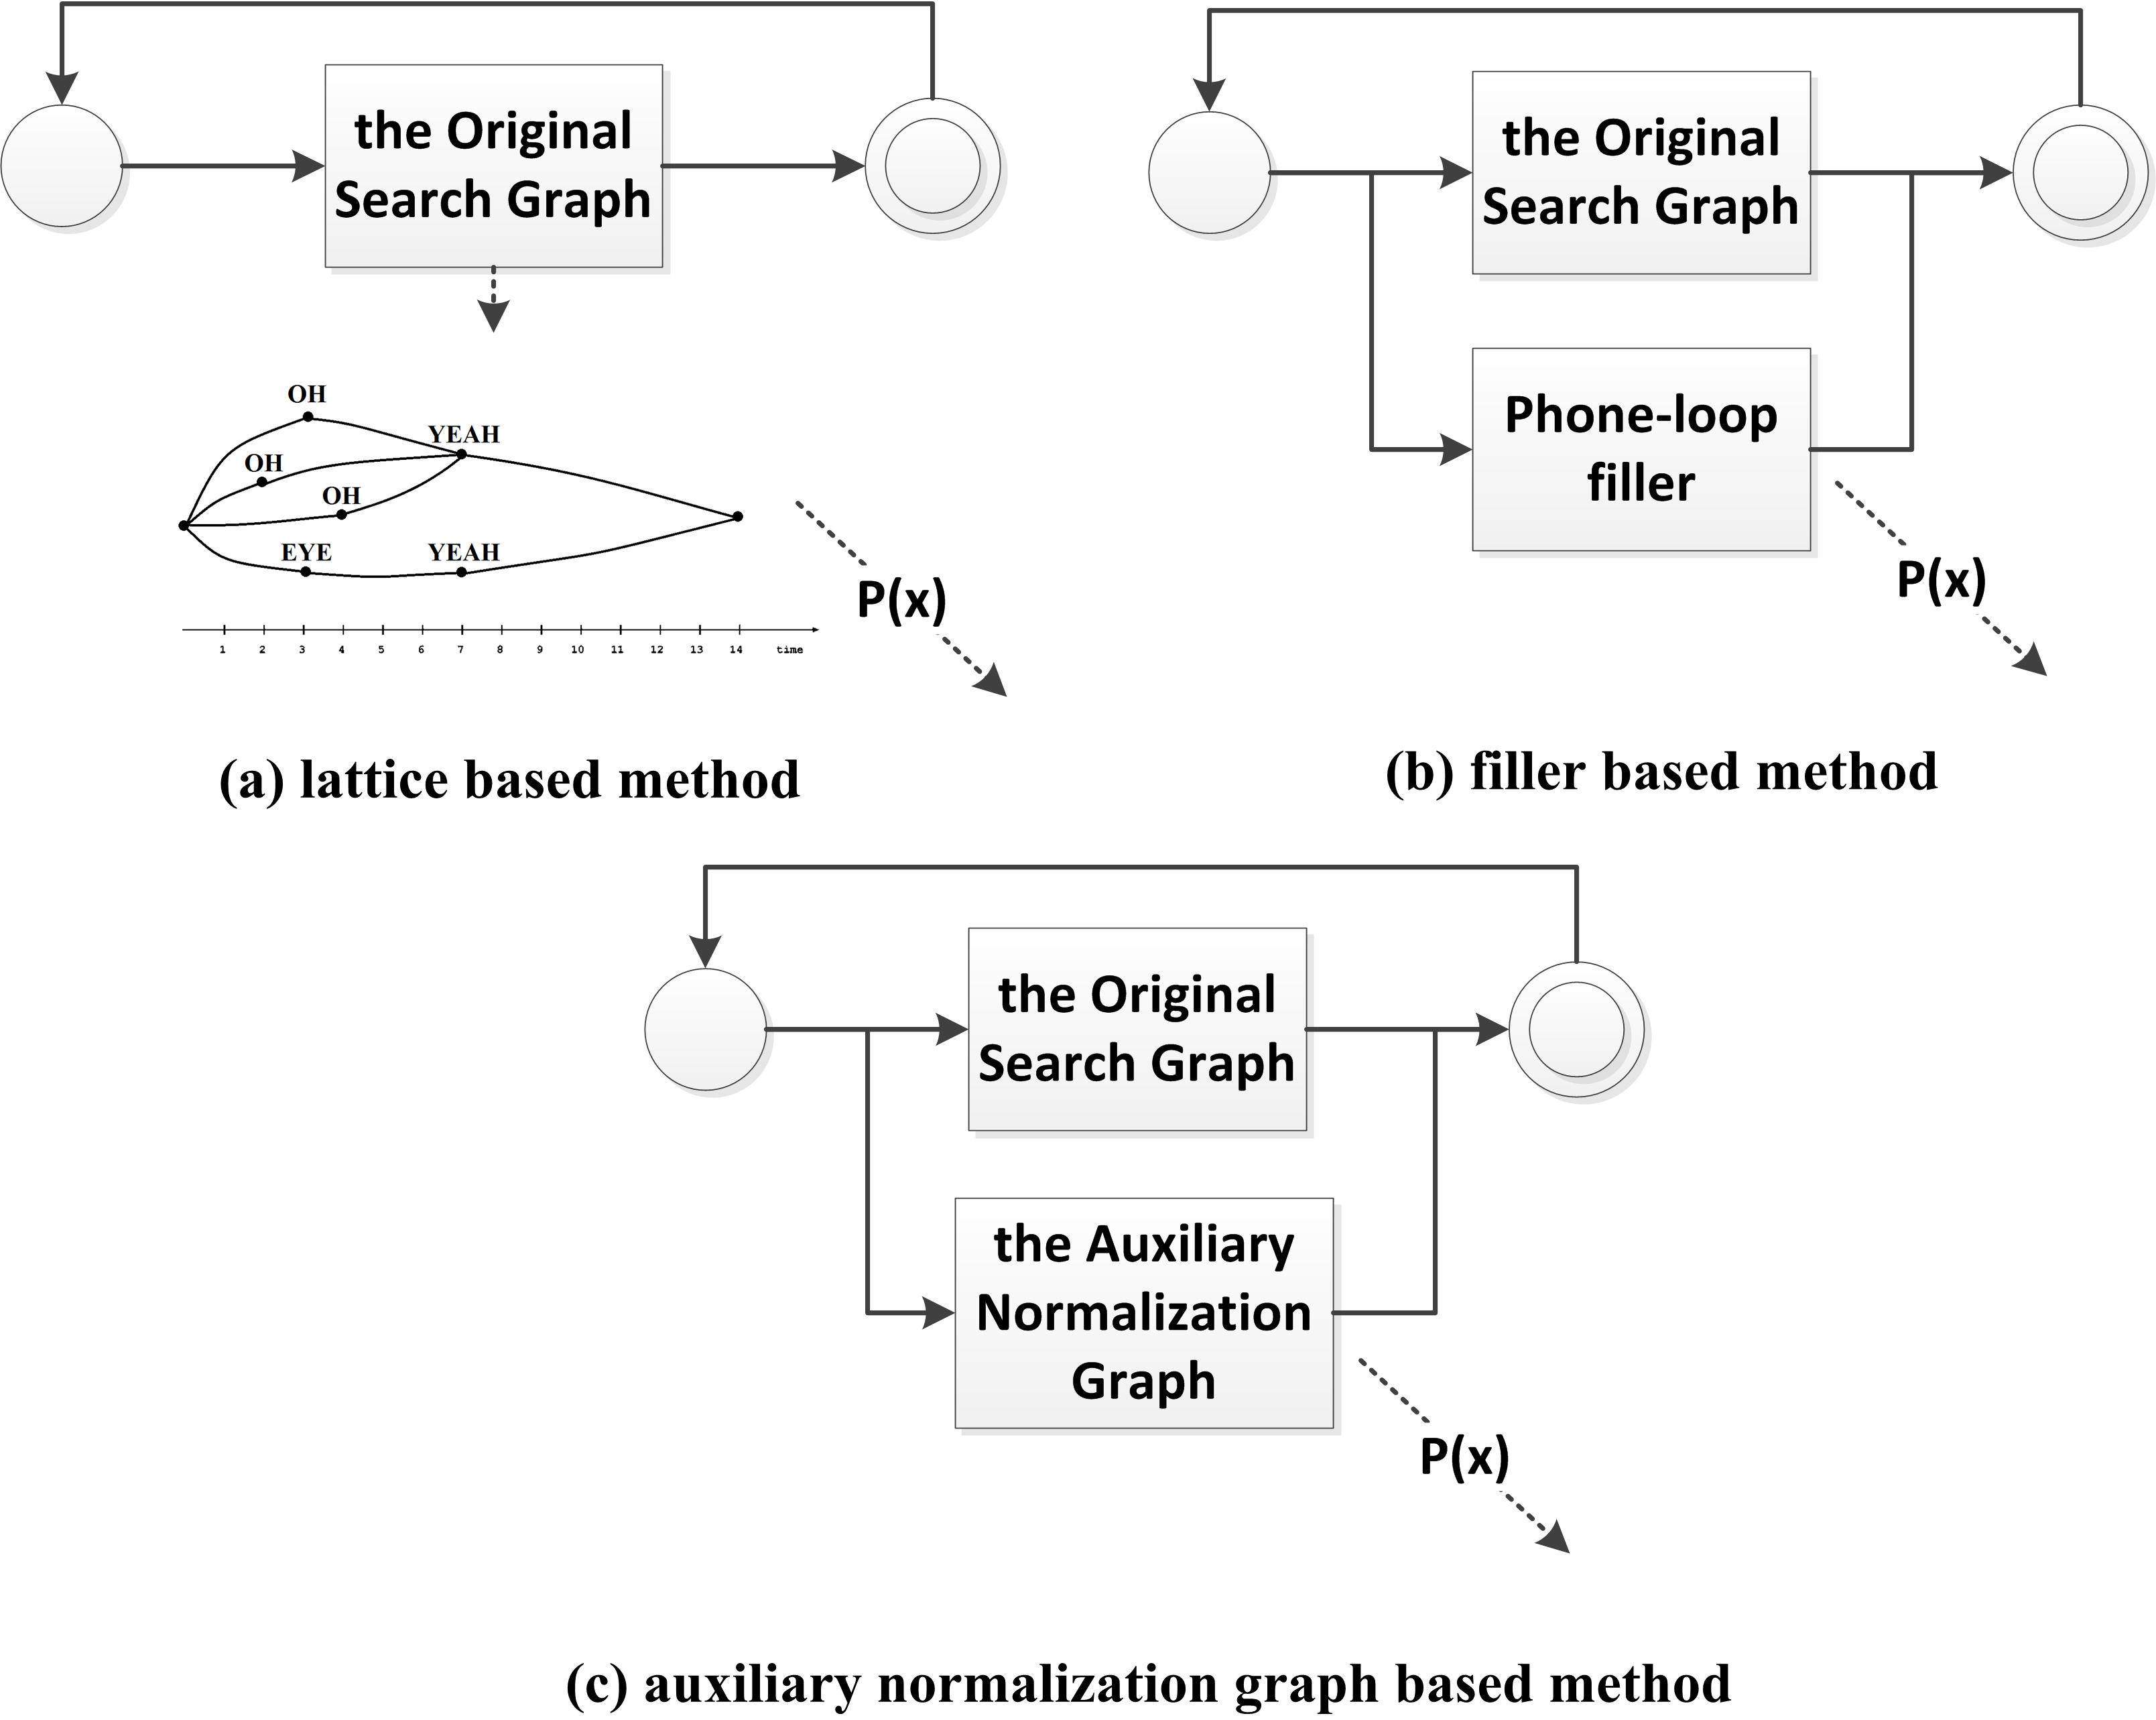
\includegraphics[width=0.7\linewidth]{figure/graph_example.png}
        \caption{{\it 架构比较。这里原始的搜索空间包括,关键词检测,基于上下文的语音识别,和大词汇连续语音识别。 }}
        \label{fig:graph-example}
\end{figure}

 \subsubsection{基于CTC的标签同步解码}
 \label{Sec:psd-ctc}

上面讨论的方法具有一定的计算昂贵性,特别是针对低功耗应用比如关键词检测。基于CTC的标签同步解码 \cite{Chen+2016} 可以考虑被采用,以加速这样的应用。由于这类方法可以跳过blank的区段,使得结果中具有更少的混淆,这体现在公式 (\ref{eq:cm-obser})中。这类方法也被前面的章节证明,解码只占全部计算量的一小部分 \cite{Chen+2016}\cite{zhc00-chen-tasl2017} 。在实验中我们将验证相关结论。



\section{基于标签同步解码的端到端语音识别}
\label{chap:lsd-e2e}

当前的端到端语音识别系统显示出诸多缺点,在开始使用标签同步解码算法进行优化之前,我们先对这些系统的缺点进行总结。

首先,声学和文本数据并不能够被系统地共同利用,这将导致声学数据的需求量非常大。
目前大多数对文本数据的应用停留于初始化阶段,但却不能在一个系统框架里,系统地使用声学和文本数据。
与之相对,传统基于深度学习的隐马尔可夫训练框架则通过贝叶斯公式,将建模拆分为声学模型,转移模型,词表和语言模型,由此进行模块化的知识源融合。

其次,声学和语言模型总是使用相同的建模单元,而这样的建模单元往往很难兼顾泛化能力和模型性能。音素感知是人类语言感知的基础单元~\cite{pisoni1985speech}。如果直接使用字符或者词作为建模单元,则并不能建立起这样的建模单元与发音之间的直接关系。这样一些研究忽略了音素这一人类语言中的先验知识。另一方面,使用字符而不是单词作为语言模型的建模单元,同样有损性能~\cite{jozefowicz2016exploring}.
%
总的来说,端到端系统建立起了与NN-HMM混合系统完全不同的一个模型框架。因此先验知识和之前在语言和声学模型方法的研究很难迁移到这一新的框架中。
%Decoding complexity. In CTC, external language model is used and increases the decoding complexity. In attention-based encoder-decoder, because the prediction in  each step is given by the last prediction, beam search is always taken to reduce the inference bias~\cite{bahdanau2015task}.

该章节将标签同步算法应用于序列到序列的端到端模型的方案。我们使用模块化训练的思想来改善端到端模型建模,使其更易于使用外在知识源来训练每一个端到端模型的子模块。值得注意的是,模型最后需要进行联合优化,因此最终在推理搜索阶段,模型仍然工作在端到端模式下。

我们为端到端模型添加的优化包括:
i) 利用声学数据和文本数据来逐一训练端到端系统,并使用模块化的策略将训练结果进行融合。具体来说先使用声学数据训练一个基于CTC的音频到音素的声学模型,而后使用文本数据训练一个基于CTC或序列到序列模型的音素到词语的语言模型。
ii) 在训练的后期,将不同模型融合为音频到词语模型,使用上文提到的标签同步解码算法对声学模型进行降采样,而后进行联合训练优化。
最终,音频到音素的声学模型,标签同步解码模块,音素到词语的语言模型被堆叠起来,在联合优化后,可以直接进行端到端推理搜索,保留了端到端系统解码简便的特性。
%
这样做的优点包括: i) 得益于模块化和初始化所带来的更简单的建模难度和更快的模型收敛速度 ii) 更易于与传统的声学建模和语言建模技术相结合,并分别使用声学和文本数据进行训练。


\subsection{训练和解码框架}
\label{sec:psd_mod_framework}

之前针对端到端语音识别的研究工作集中在将所有的模型单元融合在一起并进行联合训练和端到端解码。在这项工作中,我们提出了一种模块化的训练策略,以便优化外在知识源分别训练各个子模块的潜力。同时,我们在训练结束后仍然保留端到端解码的优点。图~\ref{fig:psd_mod_framework}显示了这一框架。


\begin{figure}
  \centering
    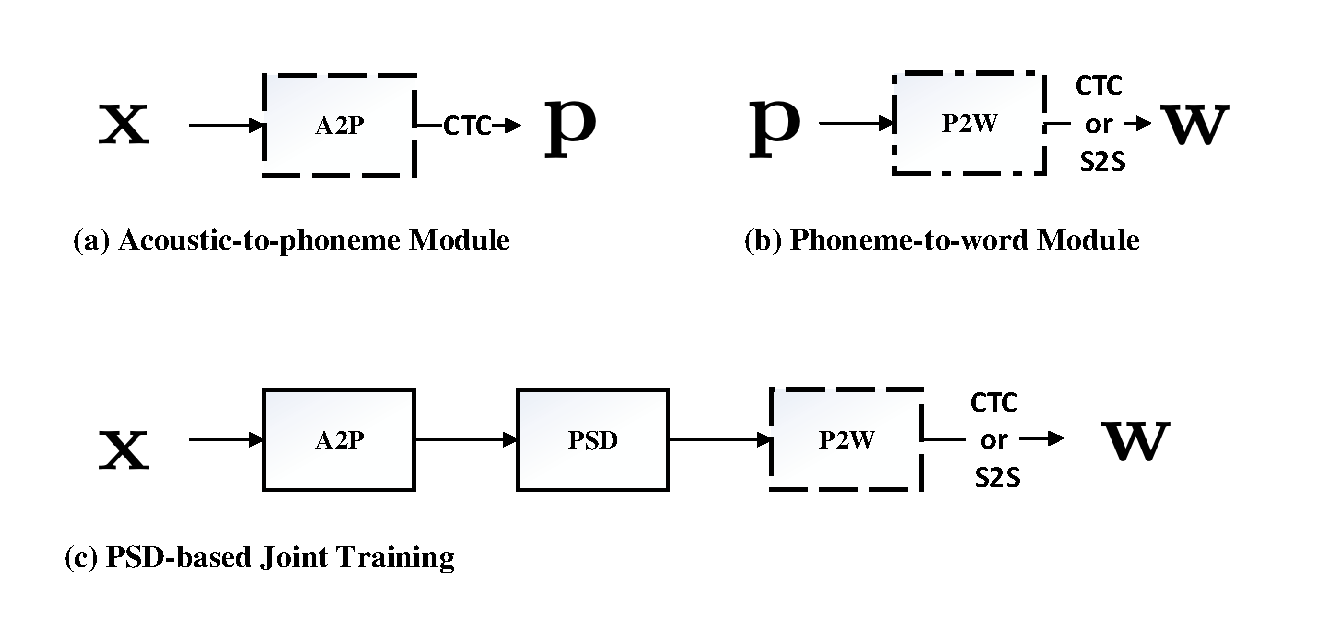
\includegraphics[width=\linewidth]{figure/psd_mod_framework.pdf}
    \caption{\it 模块化训练策略的框架。实线框表示模型参数固定不变的部分。虚线部分和点划线部分分别表示模型参数使用声学或者文本数据进行训练。}
    \label{fig:psd_mod_framework}
\end{figure}

这一端到端词序列识别系统被模块化如下:
\begin{equation}
\label{equ:framework-1}
P(\mathbf{w}|\mathbf{x})\approx\max_{\mathbf{p}} \left[\ P(\mathbf{w}|\mathbf{p}) \cdot P(\mathbf{p}|\mathbf{x})\ \right]
\end{equation}
公式中 $\mathbf{w}$, $\mathbf{p}$ 和 $\mathbf{x}$ 为词序列,音素序列和音频特征序列。
CTC准则被用于训练一个使用声学数据的声学到音素模型 (A2P)  。同时, 我们使用文本数据和CTC或S2S准则训练一个音素到词语模型。

最终各模块将被融合到一起,成为声学到词语模型 (A2W) ,在联合训练过程中我们使用了音素同步解码算法 (PSD)~\cite{zhc00-chen-tasl2017}。
\begin{equation}
\label{equ:framework-2}
P(\mathbf{w}|\mathbf{x})\approx \max_{\mathbf{p}}\left[\ P(\mathbf{w}|\mathbf{p}) \cdot PSD(\ P(\mathbf{p}|\mathbf{x})\ )\ \right]
\end{equation}
在解码阶段,经过联合训练后的模型将进行端到端推理搜索,因此其复杂度与普通端到端模型相同~\cite{audhkhasi2017direct}。
%As discussed in~\cite{audhkhasi2017direct}, the end-to-end system simplifies the decoding pipeline.  The proposed method still keeps this advantage. 

对于CTC,我们将最佳的推理搜索序列连接起来,得到最终解码序列。对于S2S模型,我们使用维特比束剪枝算法来得到相应结果。这里的端到端模型还可以进一步与外在语言模型相结合以改善性能。在这种情况下,N元语言模型将被编译为词WFST。这种情况下LSD 搜索算法~\cite{zhc00-chen-tasl2017}还可以进一步用于加速系统。


\subsection{模块化}
\label{sec:psd_mod_modu}
由于音素是人类语言重要的先验知识,它建立起了声学和语言之间的关系,因此我们采用它作为理想的建模单元。声学到音素模块使用声学数据进行训练,并预测 $P(\mathbf{p}|\mathbf{x})$ 如图~\ref{fig:psd_mod_framework}(a)所示,其与传统音素CTC建模相同~\cite{miao2015eesen}。注意的是,虽然CTC被用于该项工作,其他传统声学模型同样可以被使用,比如 RNA~\cite{sak2017recurrent} 或者 LF-MMI~\cite{povey2016purely}。

不同于传统模型,我们这里所提出的语言模型使用音素作为输入,推理搜索词序列,即 $P(\mathbf{w}|\mathbf{p})$,也就是一个音素到词的模型,如图~\ref{fig:psd_mod_framework}(b)所示。
另一个主要不同是,P2W模块使用文本和词典,不再需要使用声学数据。
总的来说,P2W模块类似于传统语言模型,除了以下几方面:

i) P2W输入的是音素序列,并隐含进行文本切分。

ii) P2W给定音素序列情况下预测词序列。因此不同于传统的语言模型专注于预测下一个词,在给定前词情况下。P2W实际上得到了更多关于下一个词的信息。因此实验结果显示,P2W的预测准确度明显高于普通的语言模型。

iii) P2W 通过序列级准则进行训练,比如CTC和S2S,这样就能够自动学习到音素和词语之间的对齐关系。


%cmp phone2graphme
我们这里同时引入了一个词边界单元 $\tt wb$ 到音素列表中,以改善文本切分效果。 $\tt wb$ 出现在词语的边界处,比如对词语 ``okay ow k ey'' ,其被修改为``okay ow k ey $\tt wb$''。 这里的想法是使用 $\tt wb$ 作为文本切分的线索,比如它可以区分一些短词可能是长词前缀的情况。

总结这里的模块化的优点包括: i) 声学和语言模型都使用了合理的建模单元 ii)系统地结果了声学和文本数据的使用来强化模型训练。


\subsection{标签同步解码}
\label{sec:psd_mod_psd}
标签同步解码在前文已进行了充分介绍,下面我们将使用它,$PSD(\cdot)$ ,作为融合系统中的一个降采样模块,应用在A2P模块上,以减少输入序列的长度。我们这样做的优点包括: i) 更短的序列减轻了LSTM进行时序建模的难度 ii)  加速了联合优化过程 iii) 该方法同时也加速了解码速度~\cite{zhc00-chen-tasl2017}.


\subsection{联合训练}
\label{sec:psd_mod_joint}
最终,所有模块将会被堆叠起来,如图~\ref{fig:psd_mod_framework}(c)所示。声学数据将用来调优该模型。
词语级别的CTC准则使用方法类似于~\cite{soltau2016neural}。
同时S2S被用于词级别的预测。在优化过程中,只有P2W进行联合训练,原因是:i) A2P工作在音素上,通常已经能取得较好性能~\cite{miao2015eesen,sak2015fast}. ii) 固定住A2P使得PSD可以显著减少音频帧数,加快训练速度。经过联合训练后,该模型仍工作在端到端推理搜索上,保留了优点。
%


\section{实验结果}
\label{chap:unify-exp}


\subsection{实验配置}

%In this section,  phone lattices from FSD and LSD were firstly compared, and their effects on CM were analyzed. Then experiments were held on proposed two types of CMs.

%\subsection{Experimental Setup}
%\subsubsection{Setups and Evaluation Metrics}

%%%%%%%%%%%% CM %%%%%%%%%%%%%
我们的置信度实验主要在300小时Switchboard上进行。而针对多种任务的融合框架则在后面介绍。
我们训练得到了上下文相关的状态级别HMM (CD-state-HMM) 和上下文无关的音素级别CTC (CI-phone-CTC) 。 训练的配置与解码配置和上文相似  \cite{zhc00-chen-tasl2017}。
所有的模型都使用大约 2-2.5M 参数,以便进行公平比较。
在测试中, 我们使用NIST Hub5e00 测试集的switchboard子集 (1831 句子) 。对CTC模型,我们测试FSD和LSD两种方法。
表~\ref{tab:asr-baseline} 给出了不同模型和解码框架下的基础性能,其与前文保持一致。



    \begin{table}[th]

    \caption{\label{tab:asr-baseline} {\it WER 比较}}
        \centerline{
          \begin{tabular}{ c  c  c  || c }
            \hline
            {Model Unit} &
            AM &%\multicolumn{1}{|c||}{AM} &
            Decoding &
            WER  \\
            \hline \hline
            CD-state & DNN-HMM &FSD&  16.7\\
            \hline
            \multirow{2}{*}{CI-phone}&\multirow{2}{*}{LSTM-CTC} &FSD&  18.7\\
            & &LSD&  18.8\\
            \hline
          \end{tabular}
        }

      \end{table}
%\subsubsection{ASR Baseline Performance}


%%%%%%%%%%%%%% unified %%%%%%%%%%%%%%%%

在测试针对各种ASR应用的通用融合框架时,我们在三种应用上分别进行试验:关键词检测,基于上下文的语音识别和大词汇连续语音识别。一个5000小时中文数据训练的CTC模型被用于测试,其配置与 \cite{Chen+2016}中相同。

在关键词检测中,词级别的置信度质量使用误唤醒和未唤醒错误来衡量。在基于上下文的语音识别中,使用句子级别的置信度来区分上文中介绍的领域内错误和领域外错误。
 {\em 等错误率} (EER) 用来度量上面两张测试下的错误率,该指标反映了误唤醒和未唤醒错误的均值。越低的EER表示越好的模型性能。
 {\em 归一化交叉熵 } (NCE) \cite{zhc00-chen-icassp2017} 用来作为词级别置信度质量的评估,在大词汇连续语音识别中。越大的NCE表示模型性能越好。为了保证ASR准确率没有受到该框架的影响,我们还度量了前两个测试中的句子的召回率,以及 在大词汇连续语音识别中的 {\em 字错误率} (CER) 。 
 为了度量框架的效率,我们给出了解码搜索时间占总体计算时间的比例,表示为 {\em portion of time except acoustic model} (PEA)。因为实验总是在相同的声学模型上进行,越低的PEA表示计算过程越少消耗在解码框架上,这包括搜索空间解码,词图生成,后处理等。因此越低的PEA效果越好。

 在基线置信度方法中包含针对用于建模的特征的置信度,表示为 $\tt AC $ 和 $ \tt CN $。 我们提出的方法分别在实验中进行了比较,他们是$\tt AX1 $, $\tt AX2 $ 和 $\tt AX3 $ 。 
 附属归一化搜索空间 $\tt AX2 $是由一个三元音素级语言模型而得到的,它包含了{\em 145K} 组词历史。 $\tt AX3 $ 是由词级别搜索网络 $L$ 与一个由所有发音自环组成的网络$G$合成得到的,  $L \circ G$. $\tt filler$ 方法没有被包括在评估中,因为它理论上和 $\tt AX1$相同。

\subsection{基于FSD和LSD的混淆网络比较}
\label{sec:exp-lattice-ana}

本章研究了LSD生成的混淆网络的质量比FSD好的原因。我们首先比较了音素词图质量,而后讨论了词级词图和混淆网络的生成方案。


\subsubsection{音素级词图质量分析}

如前面章节所讨论,CTC 模型尝试对多对一函数$\mathcal{B}$进行建模,使得最终结果能得到非常突出的音素推理搜索结果。
LSD音素词图是从丢弃了一定数量的 $\tt blank$ 帧的推理搜索分布中生成得到的,之后可以将剩余帧的一定阈值以内的音素后验概率收集起来组成时间上不连续的词语串。这样的方式避免了一些搜索错误和混淆的音素边界问题,使得最终得到的词图更紧致。

%Then, the compactness and precision of phone lattices from different frameworks were compared.
{\em 全局最优音素错误率} (OPER) 被用来对音素词图的质量进行评估。它使用词图中最优的一条路径计算得到的错误率来作为全局错误率\cite{hoffmeister2006frame}。 {\em 词图密度} (Arcs/Sec) 则被用来衡量词图的紧致程度\cite{woodland1994large}。

\begin{figure}[tbhp!]
        \centering
        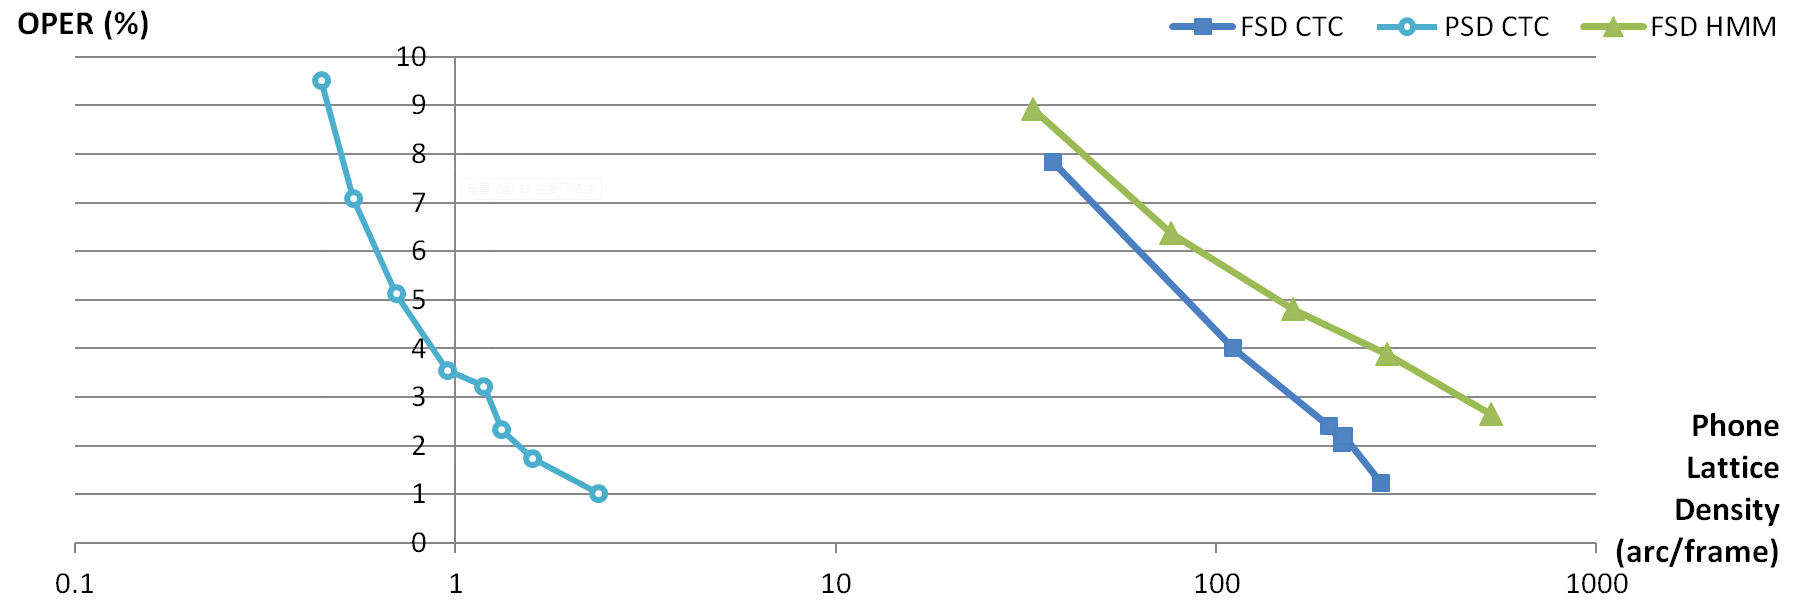
\includegraphics[width=\linewidth]{figure/OPER-latden.png}

        \caption{{\it OPER v.s. 词图密度在 FSD 和 LSD 中的比较}}
        \label{fig:OPER-latden}
      \end{figure}

图~\ref{fig:OPER-latden}表示了 OPER 和词图密度在不同解码配置结果中的对比,这包括由FSD和LSD生成的音素词图。
%Phone lattice generated from LSD is called LSD CTC lattice as in Section~\ref{sec:psd-ctc-lat} . Phone lattice generated from FSD is as the traditional method \cite{povey2012generating}.
在相似OPER情况下,对同一个CTC模型,LSD词图的大小比FSD词图小超过10倍。而LSD词图比HMM-DNN缩小的数量更大。产生这样现象的原因包括两方面:CTC更突出的后验概率特性而得到的紧致词图;LSD避免了词图生成过程的大量 $\tt blank$ 帧,而FSD则需要进行一些近似 \cite{ljolje1999efficient} 或进行词图裁剪\cite{povey2012generating}, 这将导致更大的搜索误差。
总结起来,在相同大小下,LSD CTC包含更多的音素声学信息。由于接下来的重点是比较FSD和LSD,因此我们仅罗列该部分结果。


\subsubsection{LSD CTC 词图及其生成的更好混淆网络}

%CTC model encodes the many-to-one function of $\mathcal{B}$ and results in peaky phonemic inference results.
%However, in FSD designed for HMM framework, phonemic output lasts for several frames because of  HMM modeling and state transition.  During generating word lattice, many-to-one function still needs to be done by merging same labels with similar time boundary but in a heuristic method (e.g. word lattice pruning).

为了构建混淆网络,需要先生成词级词图。 图~\ref{fig:OWER-latden} 表示了词级词图质量在FSD和LSD中的对比。
我们使用OWER进行比较。在图中纵轴,我们画出了 $1-\frac{OWER}{WER}$ 的值作为OWER相对下降值,以体现词图对最终质量改善的上限。从图中可以看出,在相同词图密度情况下,LSD系统总是得到更好的OWER。
      \begin{figure}[tbhp!]
        \centering
        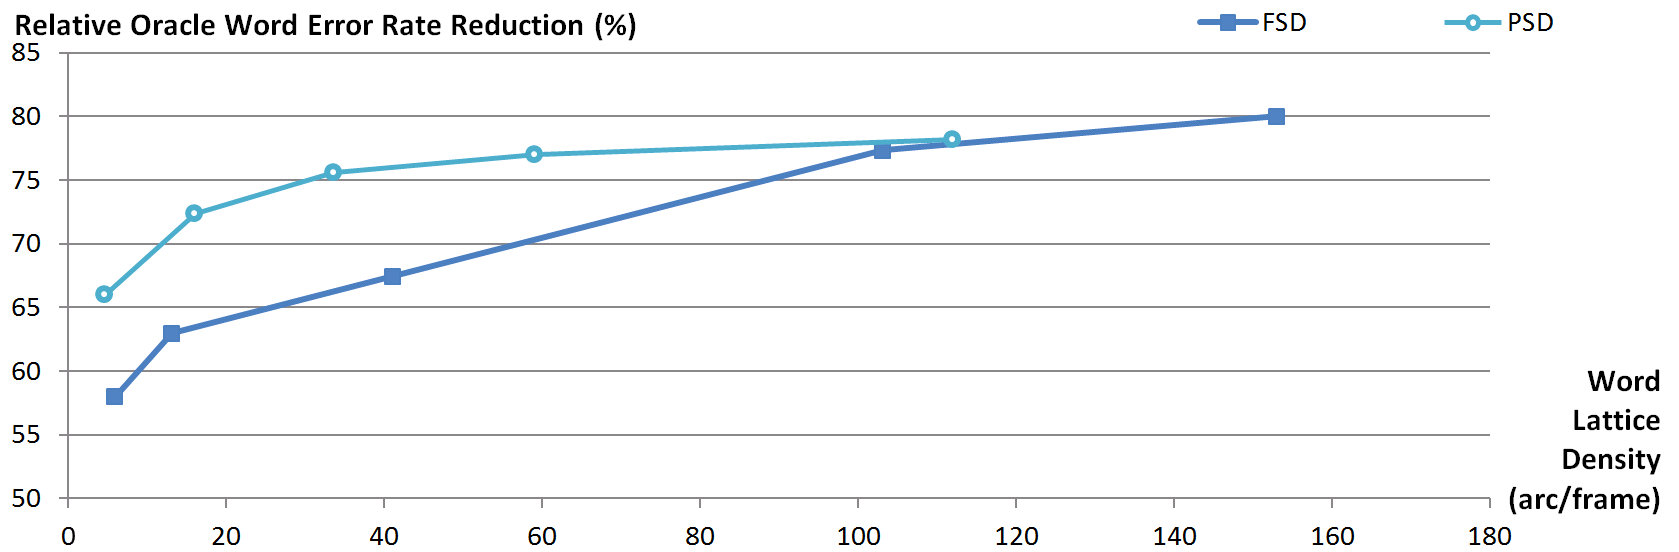
\includegraphics[width=\linewidth]{figure/OWER-latden.png}
        \caption{{\it 词图密度 v.s. 相对 OWER下降比例}}
        \label{fig:OWER-latden}
      \end{figure}
一旦词级词图被构建好,通过混淆网络的生成中的基于pivot的词聚类方法,相似时间边界的词边将会被合并在一起。因此,词级词图的时间边界的准确度对最终的混淆网络影响很大。为了分析词图的时间边界质量,我们提出最近pivot边界距离(NPBD),它定义为 $|b_{\tt arc}-b_{\tt cluster}|+|e_{\tt arc}-e_{\tt cluster}|$, 其中 $b_*$ 和 $e_*$ 为词的开始和结束时间边界, $\tt arc$ 是被对齐到最佳重叠 pivot 词 $\tt cluster$上的相应边。

%before CN cluster
      \begin{figure}[tbhp!]
        \centering
        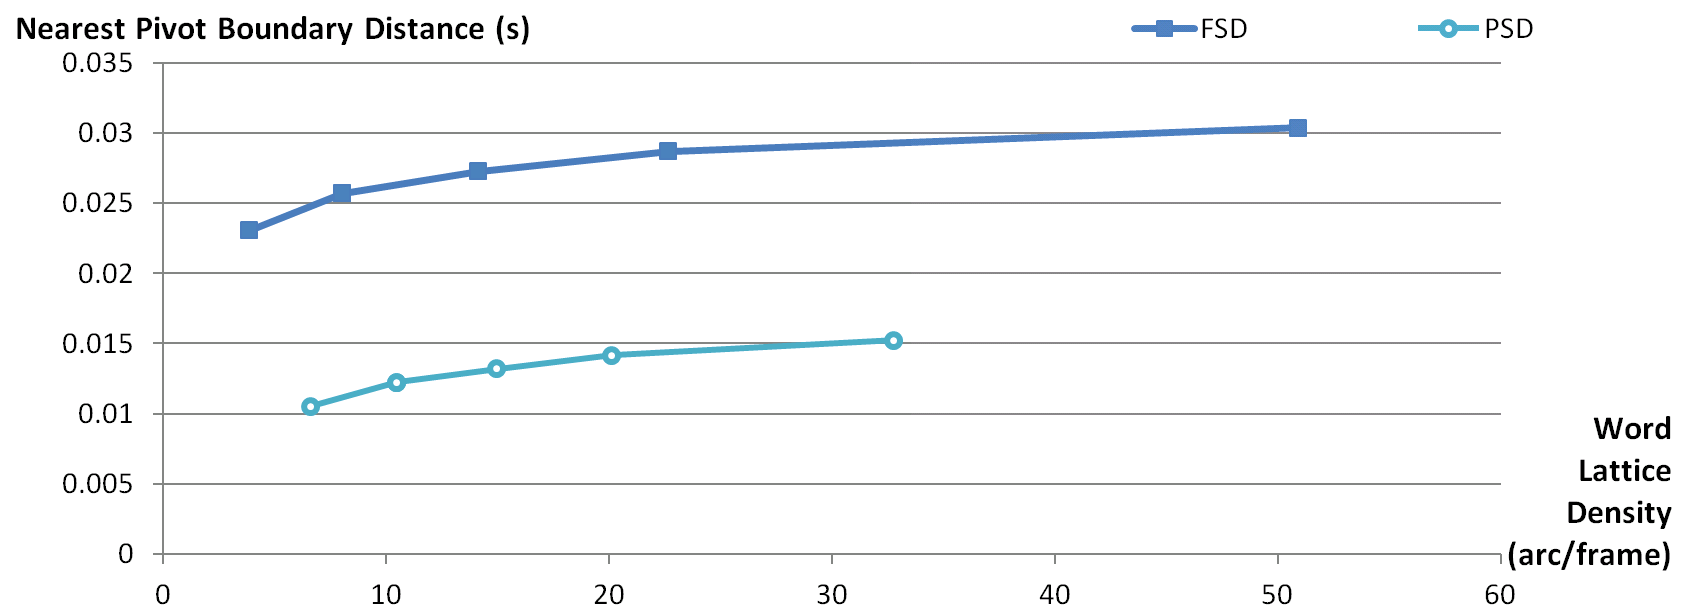
\includegraphics[width=\linewidth]{figure/bound-stable.png}
        \caption{{\it LSD和FSD的词边界稳定性}}
        \label{fig:bound-stable}
      \end{figure}
图~\ref{fig:bound-stable} 显示了LSD和FSD的NPBD。从图中可以看出LSD的词图的NPBD要明显小。换句话说,它的词边界更加稳定,由此可以得到更紧致的混淆网络。

%\subsubsection{Conversion Efficiency from Word Lattice to Confusion Network}
最后我们讨论了从词图到混淆网络的转换。图~\ref{fig:latden-cndepth} 显示了词图密度与混淆网络的深度之间的关系 \cite{hakkani2006beyond}。结果显示,即使在相似词图密度下,LSD的混淆网络往往包含更高的混淆网络深度,因此将得到更好的归一化项建模以及置信度建模方案。 

      \begin{figure}[tbhp!]
        \centering
        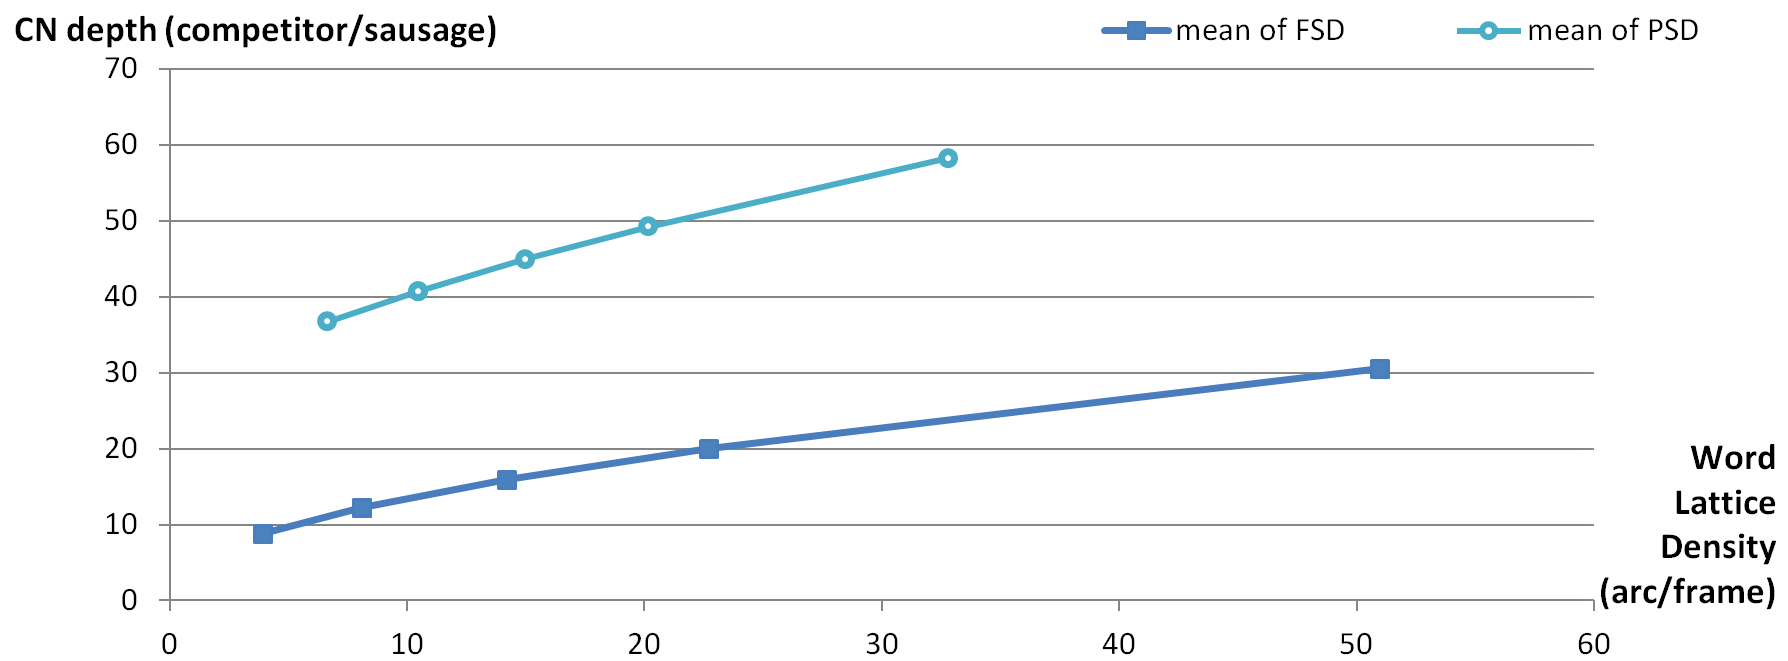
\includegraphics[width=\linewidth]{figure/latden-cndepth.png}

        \caption{{\it 词图密度 v.s. 混淆网络深度 }}
        \label{fig:latden-cndepth}

      \end{figure}


%\begin{itemize}
%    \item num of neighbors in each CN cluster(after arc clustering) from same size of lattice (in FSD \& LSD)
%    \item OWER v.s. CN size (compare FSD \& LSD)
%\end{itemize}



\subsection{置信度评估}

本章中我们比较上面讨论的混淆网络进一步得到置信度后的性能。为了补偿词图大小和对后验概率的过度估计,这里训练了一个决策树,来将所有概率映射到置信度分数上 \cite{evermann2000large}。 注意到,句子级置信度也可以由类似方法来得到。
我们使用上文提到的NCE来衡量词级置信度质量优劣。
     \begin{equation}\label{eq:nce}
    NCE=\frac{H(\mathbf{C})-H(\mathbf{C}|\mathbf{x})}{H(\mathbf{C})}
     \end{equation}
公式中 $H(\mathbf{C})$表示的是标注的序列的熵, $H(\mathbf{C}|\mathbf{x})$ 是置信度序列的熵。这是一个针对相比于总是提供平均分数的系统,其信息量增益的数量的指标。更高的NCE代表更好的系统。

\subsubsection{LSD 声学音素置信度}

表~\ref{tab:psd-conf}比较了所提出的LSD音素声学置信度与传统音素后验平均置信度。该传统方法 \cite{hu2013new}最初应用于HMM,并在本工作中拓展到 FSD的CTC 系统中 (表示为 {\em baseline}).  \ref{sec:psd-ac-conf} 提出的{\em peak-mean}, {\em peak-max}, {\em phone-mean}, {\em phone-conf} 
 等方案被表示为 {\tt PN1}, {\tt PN2}, {\tt PN3} and {\tt PC} 。
    \begin{table}[th]
    \caption{\label{tab:psd-conf} {\it 针对音素声学置信度的比较}}
        \centerline{
          \begin{tabular}{ c | c|  c ||  c }
            \hline
            \multirow{1}{*}{AM} &%\multicolumn{1}{|c||}{AM} &
            \multirow{1}{*}{Decoding} &
            \multirow{1}{*}{CM } &
            \multirow{1}{*}{NCE} \\
            %&&&\\
            \hline \hline
            DNN-HMM & FSD & baseline & 0.024 \\
            \hline
            \multirow{4}{*}{LSTM-CTC}&FSD&   baseline & 0.058\\
            \cline{2-4}
            &\multirow{3}{*}{LSD} &  $\tt PN1\oplus PN3$ & 0.105 \\
            &  & $\tt PN2\oplus PN3$ & 0.135 \\
            & &  $\tt PN2\oplus PN3\oplus PC$ & 0.141 \\
            \hline
          \end{tabular}
        }
      \end{table}
%fst-sp.ctc.sw1_fsh.o3g.kn_sp0_blk0_f_1ps_lconf10   FSD
结果显示,\cite{hu2013new}提出的音素声学置信度并不能被推广到词级。这是由于词边界的不确定性使得声学分数计算的时候存在重叠, 因此表现出了更差的结果。当该方法被使用在CTC模型时,词边界重叠问题得到了缓解,但是对于 {$\tt blank$} 概率的分配仍然存在混淆,比如对任意一个 {$\tt blank$} 是应该分配给前一个音素还是后一个音素存在不确定性。

在 LSD框架里,词边界和 {$\tt blank$} 分配问题都能够被解决,使得我们可以得到质量更好的置信度。同时当声学置信度和基于{\em phone-conf} 的置信度进行融合时,往往能取得最好的结果。因此在后续实验中,我们使用 $\tt PN2\oplus PN3\oplus PC$ 作为所提出的最优置信度。
%This is another superiority of LSD phonemic acoustic confidence because of effective usage of  information from {$\tt blank$} span.


\subsubsection{基于LSD的混淆网络的置信度}
%swb & CellPhone

%\subsubsection{Quality Comparison of Confidence Measures}
%word level NCE
表~\ref{tab:cn-conf} 比较了从LSD和FSD产生的混淆网络的置信度的质量。

    \begin{table}[th]
    \caption{\label{tab:cn-conf} {\it 基于混淆网络的置信度比较}}
        \centerline{
          \begin{tabular}{ c  |c|  c || c   }
            \hline
            \multirow{1}{*}{AM} &%\multicolumn{1}{|c||}{AM} &
            \multirow{1}{*}{Decoding} &
            \multirow{1}{*}{CM} &
            \multirow{1}{*}{NCE} \\
            %&&&\\
            \hline \hline
            DNN-HMM & FSD & \tt CN & 0.172 \\
            \hline
            \multirow{3}{*}{LSTM-CTC}&FSD&  \tt CN & 0.019\\
            \cline{2-4}
            &\multirow{2}{*}{LSD} &  \tt CN & 0.224 \\
            &  & \tt AC+CN & 0.230 \\
            \hline
          \end{tabular}
        }
      \end{table}
%kaldi get NCE
%/speechlab/users/zhc00/works/ctc/ctc-swb-ci-0621/kaldi_dec/get_nce.sh
%interpolation dir:
%/home/zhc00/new_fdecode_proj/conf_interpolation/README
%/home/zhc00/new_fdecode_proj/conf_interpolation/README_swb
%kaldi dnn get NCE
%from: zhc00@wuhan:/speechlab/users/zhc00/works/ctc/ctc-swb-ci-0621/dnn$ vi local/score_sclite_conf.sh
%zhc00@wuhan:/speechlab/users/zhc00/works/ctc/ctc-swb-ci-0621/dnn$ grep Sum exp/dnn_relu_asgd_svd/lang_decode_sw1_fsh.o3g.kn/eval2000_0.0833_10/score_*/eval2000.sw.ctm.filt.sys | awk '{print $1,$11,$14}'
%exp/dnn_relu_asgd_svd/lang_decode_sw1_fsh.o3g.kn/eval2000_0.0833_10/score_10_0.0/eval2000.sw.ctm.filt.sys:| 17.4 0.076
%exp/dnn_relu_asgd_svd/lang_decode_sw1_fsh.o3g.kn/eval2000_0.0833_10/score_12_0.0/eval2000.sw.ctm.filt.sys:| 17.0 0.139
%exp/dnn_relu_asgd_svd/lang_decode_sw1_fsh.o3g.kn/eval2000_0.0833_10/score_14_0.0/eval2000.sw.ctm.filt.sys:| 17.1 0.191
%exp/dnn_relu_asgd_svd/lang_decode_sw1_fsh.o3g.kn/eval2000_0.0833_10/score_16_0.0/eval2000.sw.ctm.filt.sys:| 17.7 0.209
%exp/dnn_relu_asgd_svd/lang_decode_sw1_fsh.o3g.kn/eval2000_0.0833_10/score_19_0.0/eval2000.sw.ctm.filt.sys:| 18.9 0.241

%fdecode result
%results/fst-sp.ctc.sw1_fsh.o3g.kn_sp0_blk2_f_1ps_nno_cn_np.nbest-10.1.car.0.0.5.eval2000.feat.fst_ctc_feat_v4/final.rst

该结果显示,虽然这种置信度在 CD-state-HMM 框架下效果较好 (与文献 \cite{evermann2000large}\cite{wessel2001confidence}一致), 但却不能够被直接应用到 CI-phone-CTC 模型上。这也是由于 {$\tt blank$} 的分配问题。
相反,基于CN的置信度可以被直接应用到LSD CTC音素词图框架并取得显著的性能改善。而且NCE还显著好于 CD-state-HMM 系统。我们相信这是因为CTC词图包含了更多的竞争信息,使得归一化项建模得更好,如图~\ref{fig:latden-cndepth}所示。

%CTC model encodes the many-to-one function of $\mathcal{B}$ and results in peaky phonemic inference results.
%However, in FSD designed for HMM framework, phonemic output lasts for several frames because of  HMM modeling and state transition.  During generating word lattice, many-to-one function still needs to be done by merging same labels with similar time boundary but in a heuristic method (e.g. word lattice pruning).

当LSD音素声学置信度 ($\tt PN2\oplus PN3\oplus PC$ 在表~\ref{tab:psd-conf}) 和基于CN的置信度相结合时 (表示为 {\tt AC+CN}), 性能得到了进一步改善。结果显示这两种置信度具有互补作用。我们认为第一种关注于局部而第二种则注重整个句子的评估。

%%%%%%%%%%%%%% unified %%%%%%%%%%%%%%%%


 \subsection{统一解码框架}
 \label{Sec:exp-kws}
 %meidi / wsj
 %EER & FScore
 在第一部分关键词检测任务中, 我们使用了398 个家居领域的关键词和相应的17332句测试集,这包括11789 个正例和 5543 个负例。表~\ref{tab:exp-kws-cm} 显示了不同方法之间的差别。

%RECALL: similar
%confidence v.s.: OK! google(bottum-up phonemic match method) & LSD lattice confidence & LSD acoustic confidence

    \begin{table}[th]

    \caption{\label{tab:exp-kws-cm} {\it KWS 任务}}

        \centerline{
          \begin{tabular}{  c|  c ||  c |c|c }
            \hline
            %\multirow{1}{*}{AM} &%\multicolumn{1}{|c||}{AM} &
            \multirow{1}{*}{CM } &
            \multirow{1}{*}{setup } &
            \multirow{1}{*}{EER(\%)} &
            \multirow{1}{*}{snt recall(\%)} &
            \multirow{1}{*}{PEA(\%)} \\
            %&&&\\
            \hline \hline
            %\multirow{2}{*}{DNN-HMM} & Phonemic  & - & 12.76 & -\\
            %\cline{2-5}
            %  & Hypothesis  & $\tt AX1$ & - & -\\
            %\hline
            Phonemic & $ \tt AC $  & 11.65 & 88.4 & 10 \\ %91.55
            \cline{1-5}
            \multirow{4}{*}{Hypothesis } &  $ \tt CN $ & 12.55 & 88.4 & 11\\
            \cline{2-5}
              & $\tt AX1$ & 11.60 & 88.0 & 10\\
              & $\tt AX2$ & 10.16 & 88.2 & 16\\
              & $\tt AX3$ & 10.10 & 88.2 & 15\\
            \hline
          \end{tabular}
        }

      \end{table}

 结果显示 $ \tt AC $ 效果比 $ \tt CN $好。原因是KWS中对搜索空间归一化项的建模非常薄弱,使得该部分估计不准。 本文所提出的附属归一化搜索空间可以减轻这样的问题,表中显示出了很大的改善。

除此之外,召回率显示本文提出的方法轻微影响了模型的准确度。考虑到在误唤醒方面显著的改善,这样的损失是可以接受的。

在效率方面,$ \tt CN $ 计算大约比 $ \tt AC $占据时间增加 10\% 。这方面来源于词图和混淆网络生成。虽然PEA比$ \tt AC $ 和 $ \tt CN $方法大, 但是总的时间仍然很小。这里的原因是由于使用了上文的LSD技术使得解码整体速度大幅加快\cite{Chen+2016}。

第二部分实验基于上下文的语音识别包含 13186 句语音助手语音,其中有7923 正例和 5263 反例。这些句子包括打电话,命令等。 这里的语法包括了所支持的说话方式和联系人信息。这里的负例包含领域内和领域外的错误。
 %dianhua
 %EER & FScore
 %RECALL: similar
    %confidence v.s.: LSD lattice confidence & LSD acoustic confidence

    \begin{table}[th]

    \caption{\label{tab:exp-grammar-cm} {\it 基于上下文的语音识别}}

        \centerline{
          \begin{tabular}{  c|  c ||  c |c|c }
            \hline
            %\multirow{1}{*}{AM} &%\multicolumn{1}{|c||}{AM} &
            \multirow{1}{*}{CM } &
            \multirow{1}{*}{setup } &
            \multirow{1}{*}{EER(\%)} &
            \multirow{1}{*}{snt recall(\%)} &
            \multirow{1}{*}{PEA(\%)}  \\
            %&&&\\
            \hline \hline
            %\multirow{2}{*}{DNN-HMM} & Phonemic  & - & 22.00 & -\\
            %\cline{2-5}
            %  & Hypothesis  & $\tt AX1$ & - & -\\
            %\hline
            %\multirow{4}{*}{LSTM-CTC}&
            Phonemic &   $ \tt AC $ & 19.86 & 87.4 & 38\\ %91.55
            \cline{1-5}
            \multirow{4}{*}{Hypothesis } &  $ \tt CN $  & 15.78  & 87.4 & 43 \\
            \cline{2-5}
              & $\tt AX1$ & 19.80  & 86.0 & 38 \\
              & $\tt AX2$ & 16.23   & 87.2 & 41\\
              & $\tt AX3$ & 16.12  & 87.2 & 40 \\
            \hline
          \end{tabular}
        }

      \end{table}

    表~\ref{tab:exp-grammar-cm} 给出了结果。在相比之前更大的搜索空间下, $ \tt CN $ 显著超越了 $ \tt AC $,因为 $ \tt AC $ 并没有使用其他的竞争信息,由此容易造成误唤醒。 $ \tt AX2 $ 和 $ \tt AX3 $ 类似于 $ \tt CN $。 原因是我们所提出的附属归一化搜索空间是针对ASR搜索空间的一个很好近似。 $\tt AX3$ 依然是性能最好的一个系统,我们将其用于下面的实验。

    关于效率,我们测试的框架对其基本没有影响。原因是与原来的搜索空间相比,我们提出的附属归一化搜索空间由于非常小,只会带来轻微影响。

    \subsection{大词汇连续语音识别}
    \label{Sec:exp-lvcsr}

    本章将在一个25小时左右的对话测试集中进行。解码使用一个118K词表的三元语言模型,其包含 {\em 1.9M} 个词对历史。
    %Table~\ref{tab:exp-lvcsr-cm} shows the result.

%RECALL: similar
    %confidence v.s.: LSD lattice confidence & LSD acoustic confidence

    \begin{table}[th]

    \caption{\label{tab:exp-lvcsr-cm} {\it LVCSR 任务}}

        \centerline{
          \begin{tabular}{  c|  c ||  c |c |c}
            \hline
            %\multirow{1}{*}{AM} &%\multicolumn{1}{|c||}{AM} &
            \multirow{1}{*}{CM } &
            \multirow{1}{*}{setup } &
            \multirow{1}{*}{NCE} &
            \multirow{1}{*}{CER(\%)} &
            \multirow{1}{*}{PEA(\%)} \\
            %&&&\\
            \hline \hline
            %\multirow{1}{*}{DNN-HMM} & Hypothesis  &  lattice based & - & -\\
            %\hline
            %\multirow{3}{*}{LSTM-CTC}&
            Phonemic &   $ \tt AC $  & 0.182& 10.2& 45  \\ %S-RTF 0.0072 RTF 0.016
            \cline{1-5}
            \multirow{2}{*}{Hypothesis } &  $ \tt CN $  & 0.302 & 10.2& 50 \\
            \cline{2-5}
              & $\tt AX3$ & 0.260 &10.1 & 46 \\
            \hline
          \end{tabular}
        }

      \end{table}

    与前面结论一致,$ \tt CN $ 性能好于 $ \tt AC $ 。 所提出的$ \tt AX3 $的结果比  $ \tt CN $差但差距不大。原因是对于LVCSR的搜索空间建模以及比较完整,附属归一化搜索空间并没有带来什么新的提升。另一方面基于效率考虑, $ \tt AX3 $使用最优路径来近似搜索空间,因此不如基于词图的建模更加完整。

    附属归一化搜索空间的系统的CER有轻微改善。我们认为是由于该搜索空间的存在将一些错误的搜索路径进行了剪枝,所以减少了插入和替换错误。关于效率,我们所提出的方法与之前一样影响不大。

    %Taking all three experiments into account, the proposed unified confidence measure and decoding framework using auxiliary normalization graph and phone synchronous decoding provides consistent performance and efficiency across varieties of ASR search space within the single framework.


\subsection{标签同步解码在模块化训练的端到端系统中的应用}
\label{exp:psd_mod}

表\ref{tab:exp-module}针对各个模块的验证集(CV)上的性能进行了比较。加粗的系统将在后续中进行使用。

\begin{table}[thbp!]
  \caption{\label{tab:exp-module} {\it  各个模块的性能比较 }}
  %\vspace{1mm}
  \centerline{
    \begin{tabular}{c c c c||m{0.15\columnwidth}}
      \hline
      模块  & 模型 & 推理搜索单元 & 词边界 & PER/WER CV (\%) \\
      \hline \hline
      \multirow{2}{0.08\columnwidth}{A2P}& \multirow{2}{0.08\columnwidth}{CTC} & \multirow{2}{0.15\columnwidth}{phoneme} & $\times$& 13.0 \\
      &  &  & $\surd$& {\bf 12.0} \\
      \hline\hline
      \multirow{4}{0.08\columnwidth}{P2W}& \multirow{2}{0.08\columnwidth}{CTC}  &\multirow{2}{0.1\columnwidth}{word}   & $\times$  &16.0 \\
      &  &  & $\surd$  &{\bf 4.3} \\
      \cline{2-5}
      & \multirow{2}{0.08\columnwidth}{S2S}  & \multirow{2}{0.1\columnwidth}{word}  & $\times$  & 13.9 \\
      &  &  & $\surd$  & {\bf 2.8} \\
      \hline
    \end{tabular}
  }
\end{table}

在A2P中,音素CTC的识别性能与~\cite{graves2006connectionist}中一致。 
%add wb didnt affect result, 
引入的$\tt wb$ 并不影响ASR性能。 
%the slight imp because Error rate of A2P phoneme with wb includes wb token
该系统中轻微的性能改善来自统计PER时包含了 $\tt wb$这一单元。而进一步统计 $\tt wb$ 的预测准则显示其低于 4\%。

在P2W模块中,CTC和S2S都进行了比较。在不包含 $\tt wb$ 情况下,二者的性能都不好。正如前文所讨论的, $\tt wb$ 可以提供音素序列切分的线索,因此CTC和S2S在包含$\tt wb$ 之后都得到了提升。
S2S一致地由于CTC,这是由于CTC中的CIA被去除,使建模能力得到增强~\cite{chan2016end}。 
不同于传统的语言模型,这里不适用PPL作为准则,原因是本系统自动推理搜索出音素与词之间的对齐关系,并使用序列准则进行训练。

%add blk modeling, both good
%bold taken for the latter exp


在第二部分中,我们比较了联合训练之后的结果,显示在表~\ref{tab:exp-joint}中。
%Table~\ref{tab:exp-joint} shows the results.
%proposed method versus the hybrid system and several end-to-end systems. 
%Notably, all systems utilize the Switchboard corpus without external sources.
为了更好地支撑这些结果,我们与近期在同一数据集上的公开结果进行比较~\cite{audhkhasi2017direct}。 
这里的不同实验配置包括:i) 添加i-vector自适应 ii)使用BLSTM iii) 语言模型使用了Fisher数据集。
因此本实验系统与~\cite{audhkhasi2017direct}中的系统包含相对 20-30\%的差距。 

\begin{table}[thbp!]
  \caption{\label{tab:exp-joint} {\it  针对是否包含模块化训练的性能比较 }}
  \centerline{
    \begin{tabular}{c |c |c m{0.15\columnwidth}||c c}
      \hline
       & E2E& \multicolumn{2}{c||}{Modularization } & \multicolumn{2}{c}{WER (\%)}\\
       Name &  Opt. & A2P&P2W & swbd & callhm \\
      \hline \hline
      %/speechlab/users/mkh96/asr/baseline/swbd/lstm/exp/plstm5/decode/eval2000_0.0833/score_13_0.0/eval2000.ctm.swbd.filt.sys
      %/fgfs/users/zhc00/works/ctc/allctc/amctc/ceam
      %exp/plstm5/decode_lang_decode_sw1_tg/eval2000_0.0833/score_12_0.0/eval2000.ctm.swbd.filt.sys
      CD-phone CE & $\times$ & HMM & WFST  &  14.9 & 27.6 \\
      %exp/plstm_ctc5/decode_sw1_tg/eval2000_0.6/
      CI-phone CTC & $\times$ & CTC & WFST  & 19.4 & 33.5 \\
      \hline\hline
       %Word CTC& $\surd$ & n/a & n/a  & 35.7 & 47.1 \\   
      \multirow{1}{0.17\columnwidth}{Word CTC}&$\surd$ & n/a & n/a  & 29.6 & 41.7 \\         
      \hline\hline
      %exp/swb.plstm_ctc5_wb.f.d2w.2d.train_tr90.3d2.tr.lstm_l2_c384_p256/decode.final.nnet/eval2000/ctm.swbd.filt.sys
      %exp/swb.plstm_ctc5_wb.f.d2w.2d.train_tr90.3h4.tr.lstm_l2_c700_p256/decode.final.nnet/eval2000/
      \multirow{2}{0.17\columnwidth}{Mod. CTC}&$\surd$ & CTC & CTC  & 24.9 & 36.5 \\   
      &$\surd$ & CTC & \ \ \ \ +WFST  & 23.0 & 35.1 \\ 
      \hline
       \multirow{1}{0.17\columnwidth}{Mod. S2S}&$\surd$ & CTC & S2S  & 31.2 & 40.5 \\   
      \hline
    \end{tabular}
  }
\end{table}

基线的混合系统 (CD-phone CE) 和音素 CTC (CI-phone CTC)系统罗列于第一和二行。他们都是通过WFST联合解码得到的。
%
CI-phone CTC 的性能比CD-phone CE差~\footnote{在更多数据情况下,CTC 性能比传统系统好~\cite{sak2015fast}。我们之前的研究也显示同样的结论 \cite{zhc00-chen-tasl2017}}, 这里的性能差距类似于之前在~\cite{audhkhasi2017direct}中的发现。
%Meanwhile, the gap between CD-phone CE and CI-phone CTC in this work is also similar to that in~\cite{audhkhasi2017direct}.
%
直接进行 A2W建模的 CTC (Word CTC)模型在第三行。它包含了音素模型初始化,但不包含GloVe初始化~\cite{audhkhasi2017direct}。
这里的性能明显差于 CI-phone CTC。该系统为不带有模块预训练的基线系统。

我们所提出的模块化训练系统 (Mod. CTC) 在第四行。
我们使用了基于标签同步解码的联合训练,该工作的具体效果将在表~\ref{tab:exp-psd} 中继续讨论。
Mod. CTC  显著改善了基线系统的性能。更好的性能来自: i) 得益于模块化和初始化所带来的更快和更好的模型收敛 ii) 更易于分别使用声学和文本数据来融合传统的声学和语音模型训练技术。

表~\ref{tab:exp-psd}显示了引入PSD算法的重要性。所有的结果都是基于一张 Titan GPU所得到。 ``fr./s.''表示每秒钟所处理的声学帧数。这里的训练加速来自两方面: i)PSD减少了后续P2W需要处理的序列长度 ii) 由于序列长度有所减小,更多的序列可以被载入GPU显存,由此可以加速并行计算。
同时,性能也有所改善。我们认为改善的结果来自于序列长度的缩短。虽然我们使用LSTM,但模型仍然很难记忆很长的序列。但是对于A2W建模,需要记忆的历史显著长于传统的 CI-phone CTC 或者混合系统。在其他一些研究中~\cite{chan2016end}也有类似的现象,而这些研究通过金字塔式的降帧率来缓解该问题。PSD是解决该问题的另一种思路。

%cmp several tricks:
%\begin{itemize}
%\item Table~\ref{tab:exp-psd} shows with or without PSD. 4 titan. speedup from larger streams \& PSD reduce seq len
%\item Table~\ref{tab:exp-add-text} shows the effect of  adding text data
%\end{itemize}

\begin{table}[thbp!]
  \caption{\label{tab:exp-psd} {\it  是否包含PSD情况下的模型性能和训练速度 }}
  \centerline{
    \begin{tabular}{c c||c c| c c}
      \hline
        && \multicolumn{2}{c|}{训练速度} &  \multicolumn{2}{c}{WER (\%)} \\
       Name & PSD & Seq./GPU&  fr./s. & swbd & callhm \\
      \hline \hline
      %exp/swb.plstm_ctc5.d2w.1a.train_tr90.3d3.tr.lstm_l2_c384_p256/log/train_nnet.log
     \multirow{2}{0.2\columnwidth}{Mod. CTC} & $\times$ &5 & 1027 & 32.0 & 42.5 \\
      %exp/swb.plstm_ctc5_wb.f.d2w.2d.train_tr90.3d2.tr.lstm_l2_c384_p256/log/iter05.tr.log
        & $\surd$ &{\bf 30} & {\bf 5851} & {\bf 24.9} &{\bf 36.5}  \\
      \hline
    \end{tabular}
  }
\end{table}

为了减轻CTC的CIA假设对模型性能所带来影响,我们实验了以下一些方案。
首先,一个从N元语言模型得到的WFST被用于与模型一起进行联合解码,其结果显示在表~\ref{tab:exp-joint}的第五行。该系统得到了一定性能提升。由此第2行与第5行的性能差距被缩减到少于 15\%。
%
另一种方法是使用S2S来代替CTC。我们提出的基于模块化训练的S2S系统 (Mod. S2S) 在表~\ref{tab:exp-joint}中最后一行。不同于在表~\ref{tab:exp-module}中的现象,S2S系统并未得到性能改善。通过进一步分析解码结果,我们发现S2S很易于受到音素识别错误的影响。经过联合优化后,S2S并不能恢复这些错误,这项观察同样见于其他研究~\cite{prabhavalkar2017comparison}。
%Especially, the acoustic signal is filled with much more noises than the phoneme sequences. 
在我们的研究中尚未包含字符级别的建模系统,原因是字符对于声学和语言建模的难度都比较大,如前文所述,音素和词语对本文的建模更加直接。


    
\section{本章小结}
\label{chap:unify-sum}
由于不同ASR应用之间不同的搜索空间大小和效率要求,当前业界最优的置信度及其相应的解码算法在不同应用上具有不同架构。针对基于词图后验概率的置信度,计算量主要集中在词图部分的边缘概率计算过程。本章节中,我们首先改善了基于CTC的后验概率置信度方案;而后我们结合前面章节对解码的大幅加速和搜索空间的优化等工作,提出一系列针对不同应用的通用置信度,并尝试将不同应用中的语音识别推理搜索过程统一到同一框架中。

,另一方面在端到端建模上取得了更快和更好的模型收敛和模型准确度